\chapter{Efficient fine-tuning and inference}

\section{The need for fine-tuning}

Language models are few-shot, or even zero-shot learners.
However, the upper bound in performance is generally set by finetuned models.
Even much smaller models, when fine-tuned on a task, can outperform bigger
models used with In-Context Learning.

So, we may still need to fine-tune models!

\subsection{Fine-tuning}

Fine-tuning is a simple (and intuitive) approach to improve a
model's performance on new tasks. In fine-tuning, we continue the training of a pretrained model on
the new (fine-tuning) data. All of the original model's weights can change

\begin{itemize}
  \item \textbf{Pros:} Allows achieving performance comparable to training from scratch. Smaller datasets can be used to change the behavior of pretrained models
  \item \textbf{Cons:} Resource intensive for large models
\end{itemize}

\section{Feature-based transfer}
We freeze the backbone model,  i.e., no gradient updates will be computed for those weights.

We add a trainable head. Only the weights of the head are updated. Optionally, we can “unfreeze" the last few layers of the backbone.

The original model is used as a feature extractor. The head uses the extracted features

\begin{itemize}
  \item \textbf{Pros:} Only changes a small fraction of all possible weights (less resource intensive). Works well when the original and the new task(s) are similar
  \item \textbf{Cons:} Complex (or more diverse) tasks require deeper changes. The performance on these tasks will be sub-optimal

\end{itemize}

\section{Problems with “classic" approaches}

Fine-tuning and feature-based transfer introduce opposite
benefits/problems. As models grow larger and tasks diversify, we typically struggle to use
one or the other approach. Other families of approaches emerged to overcome the limitations of the abovementioned techniques.  Parameter-efficient Fine-Tuning (PEFT)


\section{Parameter-efficient Fine-Tuning}

\begin{flushleft}
  \begin{minipage}{0.65\linewidth}

    Techniques used to reduce the
    computational cost required
    for the fine-tuning of models. PEFT techniques reduce the
    number of parameters to update. Among the others, there are:

    \begin{itemize}
      \item BitFit
      \item Adapter layers
      \item LoRA (Low Rank Adaptation)
      \item Prompt tuning
    \end{itemize}



  \end{minipage}%
  \hfill
  \begin{minipage}{0.3\linewidth}
    \centering
    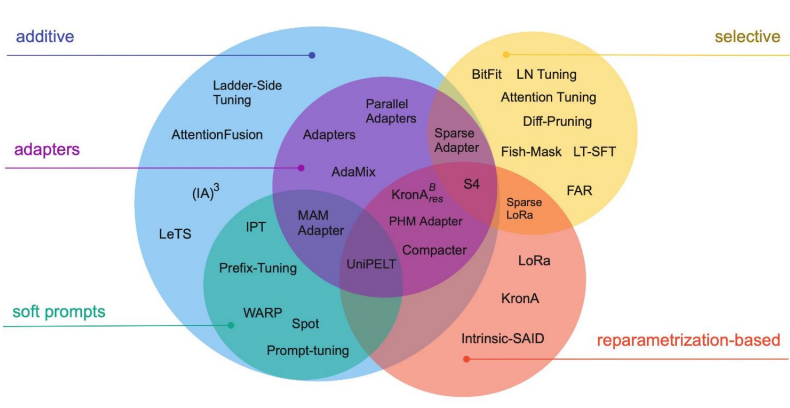
\includegraphics[width=1\linewidth]{content/Parts/images/2026-10-26-10-19-13.png}
  \end{minipage}
\end{flushleft}


\subsection{Bias-terms Fine-tuning (BitFit)}


BitFit is a very simple sparse fine-tuning technique, where only the bias terms of
the model (or a subset) are modified. Bias terms characterize a small fraction of model weights. E.g., $0.1\%$ for BERT. Zaken et al., 2021 show that tuning the bias terms is sufficient to get performance
comparable to fine-tuning. “Bias terms and their importance are rarely discussed in the literature. Indeed,
the equations in the paper introducing the Transformer model (Vaswani et al.,
2017) do not include bias terms at all, and their existence in the BERT models
might as well be a fortunate mistake"


\subsection{Adapters}

\begin{flushleft}
  \begin{minipage}{0.65\linewidth}

    Let's keep the most model freez, but add


    Introduces additional layers inbetween
    existing (attention or fully-connected) layers. Only the newly introduced layers (adapters)
    are trained. The rest of the model is frozen. Except for Layer Norms (small, and introduce
    some more flexibility). This reduces the overall number of trained
    parameters. But allows changing the model at various
    depths (unlike feature-based transfer!)


  \end{minipage}%
  \hfill
  \begin{minipage}{0.3\linewidth}
    \centering
    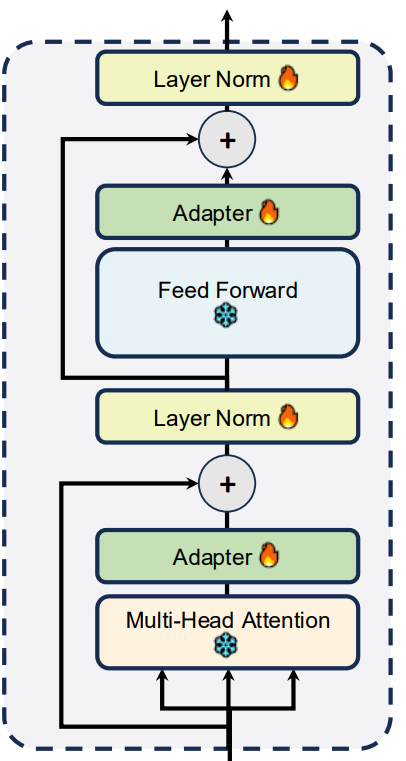
\includegraphics[width=1\linewidth]{content/Parts/images/2026-10-26-10-21-54.png}
  \end{minipage}
\end{flushleft}


\subsubsection{Adapter layer}

\begin{flushleft}
  \begin{minipage}{0.65\linewidth}

    The adapter layer is characterized by a simple
    fully-connected model


    \begin{itemize}
      \item Down-projecting layer (e.g., 768 $\to$ 32)
      \item Non-linearity (e.g., ReLU)
      \item Up-projecting layer (e.g., 32 $\to$ 768)
    \end{itemize}

    More complex architectures have been studied in
    the original paper, but with no added benefits.

    The adapters are “injected" in a pretrained (already working) model. If initialized randomly, it could “ruin" the intermediate results. Initially, the adapter should behave as an identity function ( $adapter(x) \approx$ x). Then, during fine-tuning, the layer adapts the intermediate results. To get an identity-like behavior, a residual connection is used. And the up-projecting layer is initialized with values close to 0



  \end{minipage}%
  \hfill
  \begin{minipage}{0.3\linewidth}
    \centering
    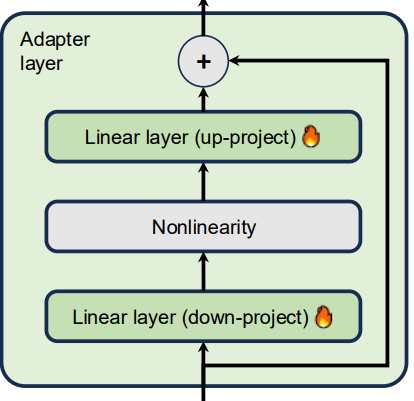
\includegraphics[width=1\linewidth]{content/Parts/images/2026-10-26-10-26-23.png}
  \end{minipage}
\end{flushleft}


\subsubsection{Results of adapters}

\begin{flushleft}
  \begin{minipage}{0.65\linewidth}

    In terms of reduction of number of trainable parameters

    A single transformer layer in BERT has ~7M parameters.
    Adapters (32 dimensions) have:

    \begin{itemize}
      \item 768*32 + 32 + 32*768+768 → ~50K parameters
      \item Two adapters for each layer → 100K parameters/layer
      \item 70x fewer parameters to tune!
    \end{itemize}

    In terms of performance:

    Authors show that, empirically, they achieve similar
    performance to using classic fine-tuning. But at a fraction of the cost!

  \end{minipage}%
  \hfill
  \begin{minipage}{0.3\linewidth}
    \centering
    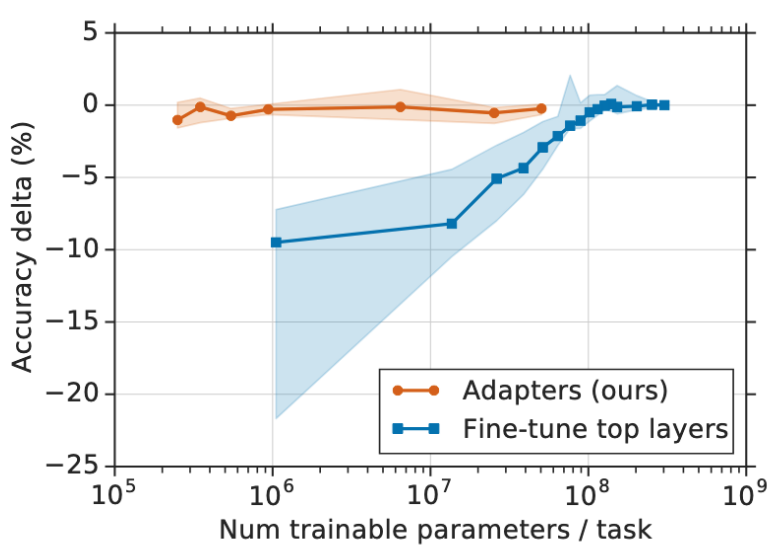
\includegraphics[width=1\linewidth]{content/Parts/images/2026-10-26-10-35-46.png}
  \end{minipage}
\end{flushleft}


\subsection{Low Ranking Adaptation (LoRA)}



\begin{flushleft}
  \begin{minipage}{0.65\linewidth}

    Fine-tuning of a model (e.g., a single layer W).
    Doing fine-tuining we update the $\delta$ produces an
    incremental change Δ𝑊 applied to the weights.

    After fine-tuning, we have new weights W'
    such that: $W' = W + \delta W$

    We can fix (freeze) W and only learn the incremental change Δ𝑊
    during fine-tuning

  \end{minipage}%
  \hfill
  \begin{minipage}{0.3\linewidth}
    \centering
    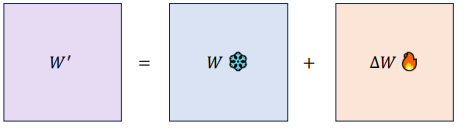
\includegraphics[width=1\linewidth]{content/Parts/images/2026-10-26-10-39-15.png}
  \end{minipage}
\end{flushleft}


\subsubsection{Rank of matrices (digression)}

The rank of a matrix is the number of linearly independent rows
(columns).
An $n \times m $ matrix $F$ is full rank if all rows (columns) are linearly
independent. It can be factorized as $F = AB^T$, both $A$ and $B$ are $n \times n$.


An $n \times n$ matrix $L$ is is low rank if some rows (columns) are linear
combinations of the other. $l =AB^T$, $A$ and $B$ are $n \times r$, with $r < n$. The rank of $L$ is $r$.


\paragraph{Low-rank factorization (digression)}

\begin{flushleft}
  \begin{minipage}{0.65\linewidth}

    This 3x3 matrix is low rank:

    \begin{itemize}
      \item row 2 = row 1 * 2
      \item row 3 = row 1 * -1
      \item rank = 1
    \end{itemize}

    It can be factorized into two 3x1 matrices

    A = [ 1 2 -1 ], B = [1 2 1]

  \end{minipage}%
  \hfill
  \begin{minipage}{0.3\linewidth}
    \centering
    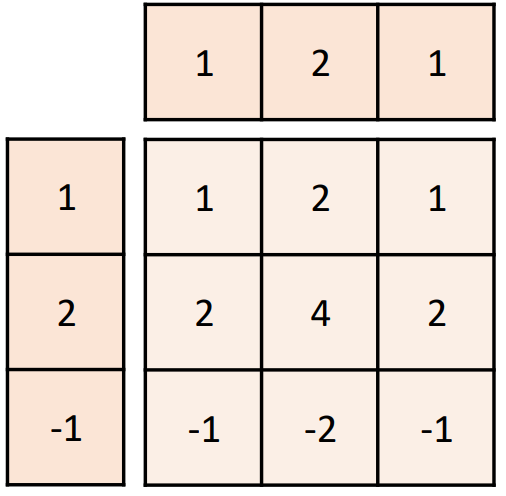
\includegraphics[width=1\linewidth]{content/Parts/images/2026-10-26-10-44-54.png}
  \end{minipage}
\end{flushleft}


\paragraph{Near low-rank (digression)}



\begin{flushleft}
  \begin{minipage}{0.65\linewidth}

    What about this matrix?
    It is technically full rank. However, it's just the previous matrix, with very small changes!. We call these matrices, near low-rank. Even if we cannot write it as $AB^T$, we can still approximate it. The closer the matrix is to actually being low rank, the better the
    approximation will be


  \end{minipage}%
  \hfill
  \begin{minipage}{0.3\linewidth}
    \centering
    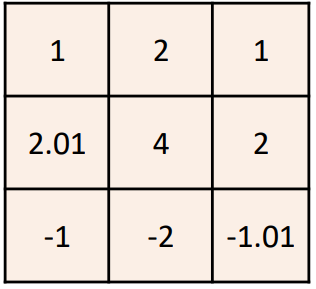
\includegraphics[width=1\linewidth]{content/Parts/images/2026-10-26-10-46-42.png}
  \end{minipage}
\end{flushleft}


\subsection{LoRA (low rank assumption of Δ𝑊)}

\begin{flushleft}
  \begin{minipage}{0.65\linewidth}


  \end{minipage}%
  \hfill
  \begin{minipage}{0.3\linewidth}
    \centering
    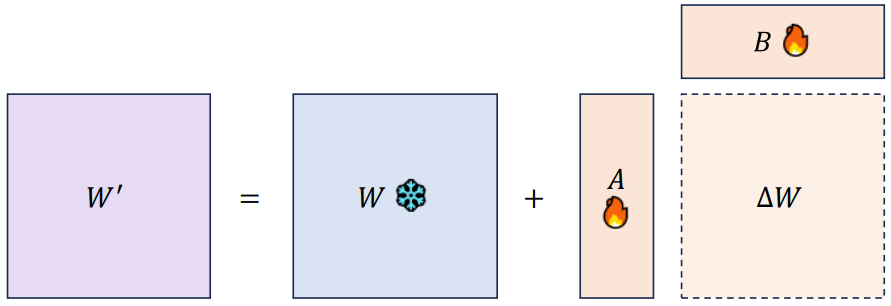
\includegraphics[width=1\linewidth]{content/Parts/images/2026-10-26-10-47-57.png}
  \end{minipage}
\end{flushleft}

\subsubsection{Low-Rank Adaptation}

\begin{equation*}
  W' = W + AB^T
\end{equation*}

Since we approximate $\delta W$, we can compute the gradients for (and optimize)
$A$ and $B$ directly.


We learn $A$, $B$ such that $AB^T$ will be approximately the desired $\delta W$.

If $\delta W$ is near low-rank, we can produce a good approximation with $A$, $B$.

So we can choose the rank to use ($r$) in the shapes of $A$, $B$.



If $r < \frac{n}{2}$, then $A$, $B$ collectively have fewer parameters than $\delta W$.

Before fine-tuning, we want $\delta W = 0$ (no update w.r.t. the pretrained model). This is achieved by sampling $A$ from $\mathcal{N}(0, \sigma^2)$ and $B = 0$ (so, $AB^T = 0)$


\subsection{Results of LoRA}
Authors show, empirically, that the
updates are indeed near low-rank.

By using values as low as r = 4, we get good approximations of $\delta W$

We can choose to fine-tune only parts of the transformer, e.g. only
queries and values, producing fewers parameters!

\subsubsection{Considerations on LoRA}
The benefits increase as we increase the model size.
with 𝑑𝑚𝑜𝑑𝑒𝑙 = 12,288 (GPT-3), we get up to 10,000x fewer parameters!
Authors claim the hardware requirements go down by a factor of 3 (forward pass still needed “in full").

We can fine-tune the same model on multiple tasks. Each task $t$ will have its $A_t$
,$B_t$ adapters.

We can store a single instance of the pretrained model, and add the
appropriate $A_t$, $B_t$ for each task needed (space efficient!)



At inference time, we can precompute $W' from W, A, B$

In this way, there's no overhead introduced by the additional
multiplications/additions required to compute $W'x = Wx + AB^T$.

\subsection{Prompt tuning}

\textbf{Prompting}: approach of adding extra information for the
model to condition on, during its generation of the output.

Normally, prompting is done by prepending some tokens to
the input, attempting to maximize the likelihood of the
correct output.

In GPT-3, for instance, these prompt tokens are
part of the model's vocabulary. In prompt design, the "right" words exist, we just need
to choose them.

In prompt tuning, instead, we add a fixed set of
special tokens to the prompt.
Then, we \textbf{allow fine-tuning only those special tokens}. (Instead of choosing the right ”words”, we create them).


\section{Other optimization techniques}

The previous techniques fall under the umbrella of PEFT. Focus on fine-tuning.

Other techniques are more generally focused on reducing the
footprint of the model. In terms of memory used, and/or computational cost. Either at training, or inference time.

This is done by either making the same model smaller. (Quantization, reduction in floating point precision). Or, by building smaller versions of models. (Distillation)



\subsection{Quantization}

Quantization is the process of mapping continuous (floating-point)
values to discrete ones.
In other words, reduce the precision of the model's weights and/or
activations by limiting the number of representable values.

\begin{itemize}
  \item \textbf{Pros:} Reduces storage/memory requirements for models. Improves computational efficiency (operations on fewer bits, possibly integer)
  \item \textbf{Cons:} Loss in precision typically has some effect on the model's performance
\end{itemize}

\subsubsection{Numerical representations }

\begin{itemize}
  \item float32: 1 bit for sign, 8 bits for exponent, 23 bits for mantissa. Range (positive): ~ $1.18 \cdot 10^{-38}$ (normalized) to $3.4 \cdot 10^{38}$
  \item float16: 1 bit for sign, 5 bits for exponent, 10 bits for fraction. Range (positive): ~ $6.1 \cdot 10^{-5}$ (normalized) to $6.5 \cdot 10^{4}$
  \item bfloat16: 1 bit for sign, 8 bits for exponent, 7 bits for mantissa. Range (positive): ~ $9.8 \cdot 10^{-4}$ (normalized) to $3.4 \cdot 10^{38}$
  \item int8: -128 to 127
\end{itemize}

\section{Quantization process}


\begin{flushleft}
  \begin{minipage}{0.65\linewidth}

    Mapping scheme.
    Specifies how values from one domain (e.g. values of a
    tensor, in float32) should map to the target domain (e.g. int8).
    Various approaches (e.g., absmax, zero-point).
    All based on scale (size of step) and zero-point (what is "0"?)

    \begin{itemize}
      \item \textbf{Absmax quantization}: Scale values symmetrically.
            If a is the abs-largest value in the tensor, values are mapped
            so as -a = -127, +a = +127.
            The original value “0” is preserved to “0” in the quantized
            version
      \item \textbf{Zero-point quantization}: Scale values asymmetrically. If min = a, max = b, values are mapped so that a = -128, b =
            +127. More efficient use of the range of possible values for
            asymmetric distributions

    \end{itemize}

  \end{minipage}%
  \hfill
  \begin{minipage}{0.3\linewidth}
    \centering
    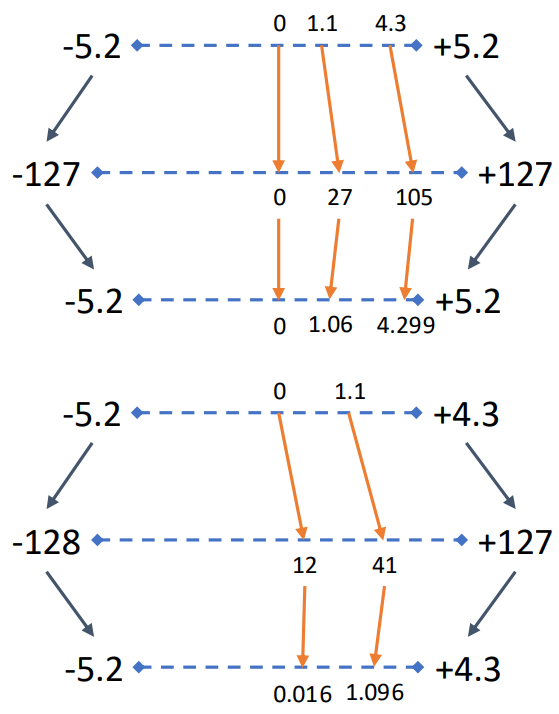
\includegraphics[width=1\linewidth]{content/Parts/images/2026-10-26-11-12-55.png}
  \end{minipage}
\end{flushleft}

\subsection{Types of quantization}

\begin{flushleft}
  \begin{minipage}{0.65\linewidth}

    \begin{itemize}
      \item \textbf{Post-Training Quantization (PTQ)}:  A model is trained “normally”, its weights and/or activations are quantized afterwards. Easy to apply to a model without retraining, but can produce sub-optimal results
      \item \textbf{Quantization-Aware Training (QAT)}:  Incorporates quantization during training.
            Forward pass.
            Using (fake) quantized version of weights/activations.
            All values are kept to full precision (but rounded).
            Backward pass.
            Gradients computed in full precision.
            Quantization parameters (e.g., scale, zero-point) are learned.
            Some tricks to bypass non-differentiable functions (e.g., rounding).
            Better performance, but requires intervening on the training process
    \end{itemize}


  \end{minipage}%
  \hfill
  \begin{minipage}{0.3\linewidth}
    \centering
    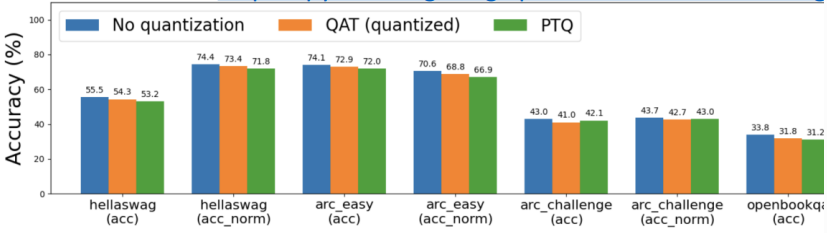
\includegraphics[width=1\linewidth]{content/Parts/images/2026-10-26-11-25-55.png}
  \end{minipage}
\end{flushleft}


\subsection{Static vs dynamic quantization}

To quantize weights/activations, we need to know scale and zero-point

For \textbf{weights}, we can compute the information beforehand
For \textbf{activations}, there are two approaches: static & dynamic quantization

\subsubsection{Static quantization}
Pre-compute scale, zero-point, then used them in a fixed way. A validation set is used to measure distributions (calibration phase). Faster, more consistent

\subsubsection{Dynamic quantization}
Compute scale and zero-point for each activation separately.
Makes better use of the range of possible values.
No calibration step required.
More computationally expensive (at inference, we compute values on the activations)



















